%! \usepackage{amsmath, amssymb, mathtools, braket}
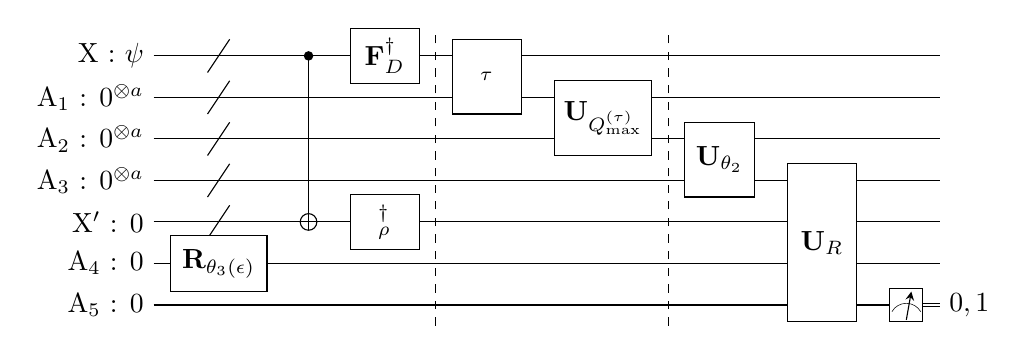
\begin{tikzpicture}[scale=1.000000,x=1pt,y=1pt]
\filldraw[color=white] (0.000000, -7.500000) rectangle (284.000000, 97.500000);
% Drawing wires
% Line 3: inputstate W \Ket{\psi}^X
\draw[color=black] (0.000000,90.000000) -- (284.000000,90.000000);
\draw[color=black] (0.000000,90.000000) node[left] {X : $\Ket{\psi}$};
% Line 4: qtau W \Ket{0}^{\otimes a}
\draw[color=black] (0.000000,75.000000) -- (284.000000,75.000000);
\draw[color=black] (0.000000,75.000000) node[left] {A$_1$ : $\Ket{0}^{\otimes a}$};
% Line 5: qtaunormalized W \Ket{0}^{\otimes a}
\draw[color=black] (0.000000,60.000000) -- (284.000000,60.000000);
\draw[color=black] (0.000000,60.000000) node[left] {A$_2$ : $\Ket{0}^{\otimes a}$};
% Line 6: theta W \Ket{0}^{\otimes a}
\draw[color=black] (0.000000,45.000000) -- (284.000000,45.000000);
\draw[color=black] (0.000000,45.000000) node[left] {A$_3$ : $\Ket{0}^{\otimes a}$};
% Line 7: aux W \Ket{0}^{X^\prime}
\draw[color=black] (0.000000,30.000000) -- (284.000000,30.000000);
\draw[color=black] (0.000000,30.000000) node[left] {X$'$ : $\Ket{0}$};
% Line 8: lambda W \Ket{0}
\draw[color=black] (0.000000,15.000000) -- (284.000000,15.000000);
\draw[color=black] (0.000000,15.000000) node[left] {A$_4$ : $\Ket{0}$};
% Line 9: cos W \Ket{0} {0,1}
\draw[color=black] (0.000000,0.000000) -- (272.000000,0.000000);
\draw[color=black] (272.000000,-0.500000) -- (284.000000,-0.500000);
\draw[color=black] (272.000000,0.500000) -- (284.000000,0.500000);
\draw[color=black] (0.000000,0.000000) node[left] {A$_5$ : $\Ket{0}$};
% Done with wires; drawing gates
% Line 11: inputstate qtau qtaunormalized theta aux /
\draw (19.500000, 84.000000) -- (27.500000, 96.000000);
\draw (19.500000, 69.000000) -- (27.500000, 81.000000);
\draw (19.500000, 54.000000) -- (27.500000, 66.000000);
\draw (19.500000, 39.000000) -- (27.500000, 51.000000);
\draw (19.500000, 24.000000) -- (27.500000, 36.000000);
% Line 16: lambda G $\mathbf{R}_{\theta_3\left(\epsilon\right)}$ width=35 height=20
\begin{scope}
\draw[fill=white] (23.500000, 15.000000) +(-45.000000:24.748737pt and 14.142136pt) -- +(45.000000:24.748737pt and 14.142136pt) -- +(135.000000:24.748737pt and 14.142136pt) -- +(225.000000:24.748737pt and 14.142136pt) -- cycle;
\clip (23.500000, 15.000000) +(-45.000000:24.748737pt and 14.142136pt) -- +(45.000000:24.748737pt and 14.142136pt) -- +(135.000000:24.748737pt and 14.142136pt) -- +(225.000000:24.748737pt and 14.142136pt) -- cycle;
\draw (23.500000, 15.000000) node {$\mathbf{R}_{\theta_3\left(\epsilon\right)}$};
\end{scope}
% Line 13: aux C inputstate
\draw (56.000000,90.000000) -- (56.000000,30.000000);
\begin{scope}
\draw[fill=white] (56.000000, 30.000000) circle(3.000000pt);
\clip (56.000000, 30.000000) circle(3.000000pt);
\draw (53.000000, 30.000000) -- (59.000000, 30.000000);
\draw (56.000000, 27.000000) -- (56.000000, 33.000000);
\end{scope}
\filldraw (56.000000, 90.000000) circle(1.500000pt);
% Line 14: aux G $\mathcal{O}_\rho^\dag$ width=25 height=20
\begin{scope}
\draw[fill=white] (83.500000, 30.000000) +(-45.000000:17.677670pt and 14.142136pt) -- +(45.000000:17.677670pt and 14.142136pt) -- +(135.000000:17.677670pt and 14.142136pt) -- +(225.000000:17.677670pt and 14.142136pt) -- cycle;
\clip (83.500000, 30.000000) +(-45.000000:17.677670pt and 14.142136pt) -- +(45.000000:17.677670pt and 14.142136pt) -- +(135.000000:17.677670pt and 14.142136pt) -- +(225.000000:17.677670pt and 14.142136pt) -- cycle;
\draw (83.500000, 30.000000) node {$\Or_\rho^\dag$};
\end{scope}
% Line 15: inputstate G $\mathbf{F}_D^\dag$ width=25 height=20
\begin{scope}
\draw[fill=white] (83.500000, 90.000000) +(-45.000000:17.677670pt and 14.142136pt) -- +(45.000000:17.677670pt and 14.142136pt) -- +(135.000000:17.677670pt and 14.142136pt) -- +(225.000000:17.677670pt and 14.142136pt) -- cycle;
\clip (83.500000, 90.000000) +(-45.000000:17.677670pt and 14.142136pt) -- +(45.000000:17.677670pt and 14.142136pt) -- +(135.000000:17.677670pt and 14.142136pt) -- +(225.000000:17.677670pt and 14.142136pt) -- cycle;
\draw (83.500000, 90.000000) node {$\mathbf{F}_D^\dag$};
\end{scope}
% Line 17: inputstate qtau qtaunormalized theta aux lambda cos TOUCH style=dashed
\draw[dashed] (102.000000,-7.500000) -- (102.000000,97.500000);
% Line 18: qtau inputstate G $\mathcal{O}_\tau$ width=25 height=20
\draw (120.500000,90.000000) -- (120.500000,75.000000);
\begin{scope}
\draw[fill=white] (120.500000, 82.500000) +(-45.000000:17.677670pt and 19.091883pt) -- +(45.000000:17.677670pt and 19.091883pt) -- +(135.000000:17.677670pt and 19.091883pt) -- +(225.000000:17.677670pt and 19.091883pt) -- cycle;
\clip (120.500000, 82.500000) +(-45.000000:17.677670pt and 19.091883pt) -- +(45.000000:17.677670pt and 19.091883pt) -- +(135.000000:17.677670pt and 19.091883pt) -- +(225.000000:17.677670pt and 19.091883pt) -- cycle;
\draw (120.500000, 82.500000) node {$\Or_\tau$};
\end{scope}
% Line 19: qtaunormalized qtau G $\mathbf{U}_{Q_{\max}^{\left(\tau\right)}}$ width=35 height=20
\draw (162.500000,75.000000) -- (162.500000,60.000000);
\begin{scope}
\draw[fill=white] (162.500000, 67.500000) +(-45.000000:24.748737pt and 19.091883pt) -- +(45.000000:24.748737pt and 19.091883pt) -- +(135.000000:24.748737pt and 19.091883pt) -- +(225.000000:24.748737pt and 19.091883pt) -- cycle;
\clip (162.500000, 67.500000) +(-45.000000:24.748737pt and 19.091883pt) -- +(45.000000:24.748737pt and 19.091883pt) -- +(135.000000:24.748737pt and 19.091883pt) -- +(225.000000:24.748737pt and 19.091883pt) -- cycle;
\draw (162.500000, 67.500000) node {$\mathbf{U}_{Q_{\max}^{\left(\tau\right)}}$};
\end{scope}
% Line 20: inputstate qtau qtaunormalized theta aux lambda cos TOUCH style=dashed
\draw[dashed] (186.000000,-7.500000) -- (186.000000,97.500000);
% Line 21: theta qtaunormalized G $\mathbf{U}_{\theta_2}$ width=25 height=20
\draw (204.500000,60.000000) -- (204.500000,45.000000);
\begin{scope}
\draw[fill=white] (204.500000, 52.500000) +(-45.000000:17.677670pt and 19.091883pt) -- +(45.000000:17.677670pt and 19.091883pt) -- +(135.000000:17.677670pt and 19.091883pt) -- +(225.000000:17.677670pt and 19.091883pt) -- cycle;
\clip (204.500000, 52.500000) +(-45.000000:17.677670pt and 19.091883pt) -- +(45.000000:17.677670pt and 19.091883pt) -- +(135.000000:17.677670pt and 19.091883pt) -- +(225.000000:17.677670pt and 19.091883pt) -- cycle;
\draw (204.500000, 52.500000) node {$\mathbf{U}_{\theta_2}$};
\end{scope}
% Line 22: cos theta aux lambda G $\mathbf{U}_R$ width=25 height=20
\draw (241.500000,45.000000) -- (241.500000,0.000000);
\begin{scope}
\draw[fill=white] (241.500000, 22.500000) +(-45.000000:17.677670pt and 40.305087pt) -- +(45.000000:17.677670pt and 40.305087pt) -- +(135.000000:17.677670pt and 40.305087pt) -- +(225.000000:17.677670pt and 40.305087pt) -- cycle;
\clip (241.500000, 22.500000) +(-45.000000:17.677670pt and 40.305087pt) -- +(45.000000:17.677670pt and 40.305087pt) -- +(135.000000:17.677670pt and 40.305087pt) -- +(225.000000:17.677670pt and 40.305087pt) -- cycle;
\draw (241.500000, 22.500000) node {$\mathbf{U}_R$};
\end{scope}
% Line 23: cos M
\draw[fill=white] (266.000000, -6.000000) rectangle (278.000000, 6.000000);
\draw[very thin] (272.000000, 0.600000) arc (90:150:6.000000pt);
\draw[very thin] (272.000000, 0.600000) arc (90:30:6.000000pt);
\draw[->,>=stealth] (272.000000, -5.400000) -- +(80:10.392305pt);
% Done with gates; drawing ending labels
\draw[color=black] (284.000000,0.000000) node[right] {${0,1}$};
% Done with ending labels; drawing cut lines and comments
% Done with comments
\end{tikzpicture}
